\chapter{Implementation}
\label{Implementation}

In this chapter, we are going to explain the major problems that we encountered during the development phase.

Addressing the client, in the \chapref*{Technologies} we already named the key frameworks and techniques that we used in the implementation. Concerning the server, which is going to provide to the client the RESTful interface, we will cover the use cases.

\begin{figure}[!htb]
    \begin{center}
    \setlength{\fboxsep}{4pt}%
    \setlength{\fboxrule}{1pt}%
    \stackunder{\fbox{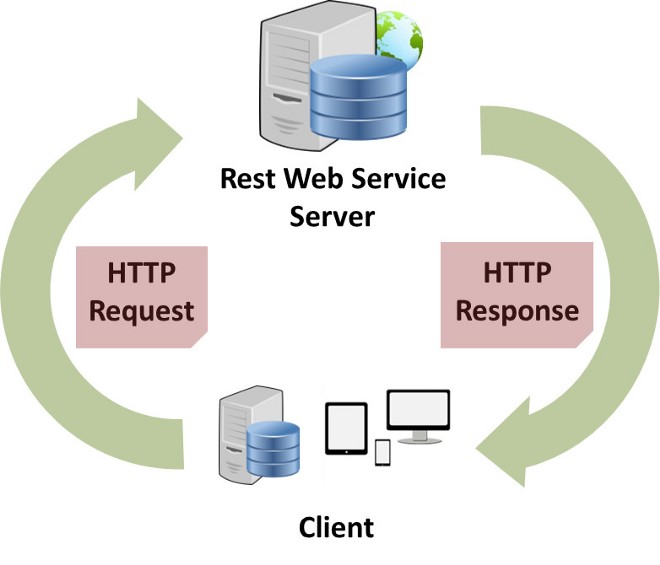
\includegraphics[width=0.5\linewidth]{images/design/clientserver.jpeg}}}%
    {\scriptsize%
     Source: \url{https://cdn-images-1.medium.com/max/660/1*EbBD6IXvf3o-YegUvRB_IA.jpeg}}
    \caption {A look at the server-client architecture with a RESTful interface.}
    \label{fig:design1}
\end{center}
\end{figure}

To demonstrate the functionality of the WebCure, we covered three different types of CRDTs: a counter, a set and a multi-value register. We managed to support each of these data types on the server and the client as well.idb.js

\begin{figure}[!htb]
    \begin{center}
    \def\svgwidth{\linewidth}
    \input{images/implementation/3tier.pdf_tex}
    \caption {3-Tier architecture.}
    \label{fig:dev1}
\end{center}
\end{figure}



\section{Server}

This part is an important part of the WebCure, as it provides the interface for the client and operates with the database layer as well. 

\section{Client}












\section{Optimization}




\begin{itemize}
    \item{The request to the server is succesfull: in this case, the request would end up changing the data on the server's side, while the client will just update its own cache once it gets a response from the server.}
    \item{The request to the server is not succesfull: here, it is going to be a bit more interesting. We will have to wait for an error message and store the data in a temporary database for the updates that are not sent to the server's side just yet. Afterwards, I think it would be logical to have a timer, which will check the connection with the server. Once it is back, every transaction again is going to be sent to the server. After all the data is sent, this temporary database can be cleaned. }
    
    \end{itemize}
    
    Several problems could arise, however, which we will adrress in the architecture chapter.